\subsubsection{Dodicesimo periodo (2024/05/30 - 2024/06/11)}
\subsubsubsection{Planning}
In questo ultimo periodo il gruppo si propone come obiettivo quello di completare tutta la documentazione in vista dell'ultima revisione. Si è quindi pianificato di scrivere una mail al prof. Cardin per fissare una data per effettuare la revisione $\textit{PB}_G$. Nel mentre, il gruppo prevede di sistemare i vari documenti per l'incontro col prof. Vardanega, cercando quindi di ottimizzare i tempi per fissare poi una data per l'interrogazione il prima possibile.
\subsubsubsubsection*{Attività pianificate}
Gli obiettivi posti per lo $\textit{sprint}_G$ sono stati i seguenti:
\begin{itemize}
    \item Effettuare il colloquio con il prof. Cardin per la revisione $\textit{PB}_G$ in data 5 giugno, per il quale si vuole:
    \begin{itemize}
        \item Preparare le diapositive per il colloquio;
        \item Preparare la lettera di presentazione per la fase $\textit{PB}_G$.
    \end{itemize}
    \item Redigere il $\textit{manuale utente}_G$;
    \item Aggiornare il documento di Analisi dei Requisiti;
    \item Aggiornare il documento $\textit{Piano di Qualifica}_G$;
    \item Aggiornare il documento $\textit{Norme di Progetto}_G$;
    \item Aggiornare il documento $\textit{Piano di Progetto}_G$;
    \item Aggiornare il documento Glossario Tecnico;
    \item Approvare tutti i documenti in vista dell'interrogazione col prof. Vardanega.
\end{itemize}
\subsubsubsubsection*{Preventivo}
\begin{table}[H]
    \centering
\begin{spreadtab}{{tabular}{|c|c|c|c|c|c|c|c|}}
    \hline
    @\textbf{Membro} & @\textbf{Re} & @\textbf{Amm} & @\textbf{An} & @\textbf{Progr} & @\textbf{Proge} & @\textbf{Ve} & @\textbf{Totale} \\
    \hline
    @ Samuele V.   & 0         & 0         & 0         & 0        & 6.5   & 1     & sum(b2:g2) \\
    @ Leonardo B.  & 2         & 3.5       & 0         & 3        & 8     & 2     & sum(b3:g3) \\
    @ Riccardo Z.  & 0         & 2         & 0         & 0        & 1     & 1     & sum(b4:g4) \\
    @ Davide B.    & 3         & 7.5       & 1         & 2.5      & 5     & 3     & sum(b5:g5) \\
    @ Michele Z.   & 3.5       & 3         & 0         & 5        & 4.5   & 8     & sum(b6:g6) \\
    @ Filippo T.   & 5.75      & 10        & 0         & 5.5      & 3.5   & 6.5   & sum(b7:g7) \\
    \hline
    @\textbf{Ore totali} & sum(b2:b7) & sum(c2:c7) & sum(d2:d7) & sum(e2:e7) & sum(f2:f7) & sum(g2:g7) &  sum(b8:g8)\\
    \hline
    @\textbf{Costo totale} & 30*b8 & 20*c8 & 25*d8 & 15*e8 & 25*f8 & 15*g8 & sum(b9:g9)\\
    \hline
\end{spreadtab}
    \caption{Preventivo orario ed economico parziale per il dodicesimo periodo, in base al ruolo}
    \vspace{5mm}
    \textbf{Legenda:} \textit{Re} = Responsabile, \textit{Amm} = Amministratore, \textit{An} = Analista, \textit{Progr} = Programmatore, \textit{Proge} = Progettista, \textit{Ve} = Verificatore
\end{table}
\begin{figure}[H]
    \centering
    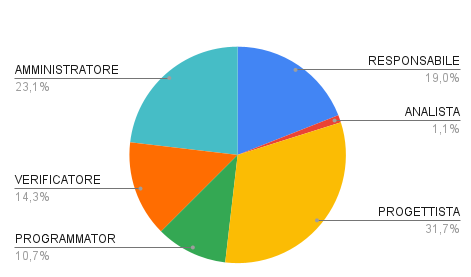
\includegraphics[width=0.6\linewidth]{grafici/12_periodo_torta.png}
    \caption{Ripartizione dei costi per ruolo nell'$12^\circ$ periodo}
        \vspace{5mm}
    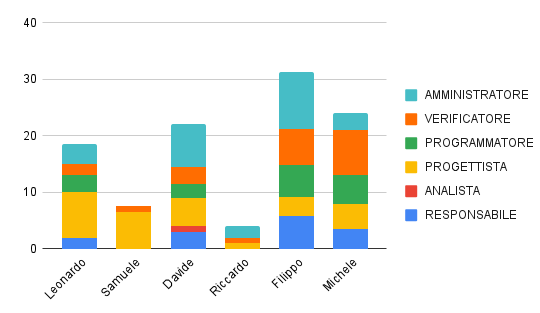
\includegraphics[width=0.7\linewidth]{grafici/12_periodo_istogramma.png}
    \caption{Ore preventivate per ciascuna persona nell'$12^\circ$ periodo}
\end{figure}
\subsubsubsection{Review}
Le attività preventivate sono state svolte con successo. La stesura e approvazione dei documenti ha richiesto più tempo di quanto sperato, nonostante ciò i tempi rientrano nelle previsioni.
\subsubsubsubsection*{Attività svolte}
Le attività svolte in questo periodo sono state le seguenti:
\begin{itemize}
    \item Effettuato l'incontro col prof. Cardin;
    \item Redatto e approvato il documento $\textit{Manuale Utente}_G$;
    \item Aggiornato e approvato il documento Analisi dei Requisiti;
    \item Aggiornato e approvato il documento $\textit{Piano di Qualifica}_G$;
    \item Aggiornato e approvato il documento $\textit{Norme di Progetto}_G$;
    \item Aggiornato e approvato il documento Glossario Tecnico;
    \item Aggiornato e approvato il documento $\textit{Piano di Progetto}_G$;
    \item Redigere la lettera di presentazione $\textit{PB}_G$ riservata alla seconda parte della revisione.
\end{itemize}

\subsubsubsubsection*{Consuntivo}
\begin{table}[H]
    \centering
\begin{spreadtab}{{tabular}{|c|c|c|c|c|c|c|c|}}
    \hline
    @\textbf{Membro} & @\textbf{Re} & @\textbf{Amm} & @\textbf{An} & @\textbf{Progr} & @\textbf{Proge} & @\textbf{Ve} & @\textbf{Totale} \\
    \hline
    @ Samuele V.   & 0        & 0         & 0         & 0         & 2.59  & 0.14  & sum(b2:g2) \\
    @ Leonardo B.  & 1.25     & 1.25      & 0         & 4         & 9.75  & 1     & sum(b3:g3) \\
    @ Riccardo Z.  & 0        & 1         & 0         & 0         & 0.5   & 0.5   & sum(b4:g4) \\
    @ Davide B.    & 3        & 8         & 1         & 2.5       & 5     & 3     & sum(b5:g5) \\
    @ Michele Z.   & 3.5      & 3.5       & 0         & 7         & 5.5   & 3.5   & sum(b6:g6) \\
    @ Filippo T.   & 6.75     & 12        & 0         & 7.75      & 2.83  & 12    & sum(b7:g7) \\
    \hline
    @\textbf{Ore totali} & sum(b2:b7) & sum(c2:c7) & sum(d2:d7) & sum(e2:e7) & sum(f2:f7) & sum(g2:g7) &  sum(b8:g8)\\
    \hline
    @\textbf{Costo totale} & 30*b8 & 20*c8 & 25*d8 & 15*e8 & 25*f8 & 15*g8 & sum(b9:g9)\\
    \hline
\end{spreadtab}
    \caption{Consuntivo orario ed economico parziale per il dodicesimo periodo, in base al ruolo}
    \vspace{5mm}
    \textbf{Legenda:} \textit{Re} = Responsabile, \textit{Amm} = Amministratore, \textit{An} = Analista, \textit{Progr} = Programmatore, \textit{Proge} = Progettista, \textit{Ve} = Verificatore
\end{table}
\begin{figure}[H]
    \centering
    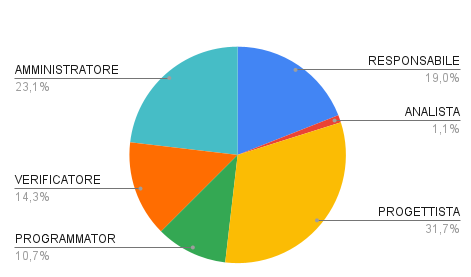
\includegraphics[width=0.6\linewidth]{grafici/12_periodo_torta_consuntivo.png}
    \caption{Consuntivo della ripartizione dei costi per ruolo nell'$12^\circ$ periodo}
        \vspace{5mm}
    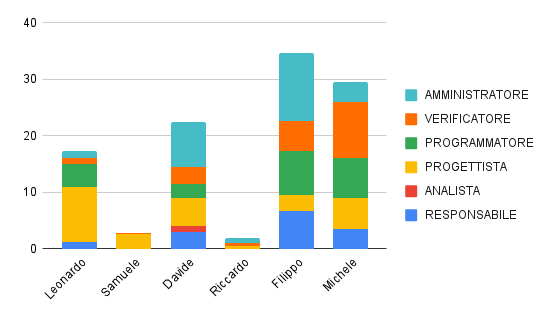
\includegraphics[width=0.7\linewidth]{grafici/12_periodo_istogramma_consuntivo.png}
    \caption{Ore eseguite per ciascuna persona nell'$12^\circ$ periodo}
\end{figure}
\subsubsubsection{Retrospective}
\paragraph*{Gestione dei Rischi}
I $\textit{rischi}_G$ occorsi per tale periodo sono stati i seguenti:
\begin{itemize}
    \item \nameref{ro:3}: Alcuni membri del gruppo, hanno avuto difficoltà a svolgere alcune task per tempo, a causa di impegni personali.
    \begin{itemize}
        \item \textbf{Esito mitigazione}: la possibilità che tale evento potesse accadere era stata notificata con anticipo, quindi si era già messo in conto un possibile ritardo nel completamento delle attività.
        \item \textbf{Impatto}: I tempi di completamento delle tasks si sono allungati, in particolar modo ha ritardato lo svolgimento di task di verifica, riguardanti documenti non ancora aggiornati.
    \end{itemize}
    \item \nameref{ro:5}: Alcuni membri del gruppo avevano da redigere documenti con cui avevano poca familiarità.
    \begin{itemize}
        \item \textbf{Esito mitigazione}: qualora qualche membro del gruppo avesse avuto difficoltà a redigere o verificare qualche documento, i membri del gruppo più liberi ed esperti erano disposti a dare una mano.
        \item \textbf{Impatto}: I tempi di completamento si sono comunque allungati un po', ma nel complesso non c'è stato un impatto negativo.
    \end{itemize}
\end{itemize}
\paragraph*{Considerazioni}
\begin{itemize}
    \item Nonostante i leggeri ritardi nell'esecuzione delle varie tasks, il gruppo è soddisfatto dei tempi di completamento degli obiettivi fissati per questo periodo.
\end{itemize}